\chapter{Complexidade de tempo}

\index{complexidade de tempo}

A eficiência dos algoritmos é importante na programação competitiva.
Normalmente, é fácil projetar um algoritmo
que resolve o problema lentamente,
mas o verdadeiro desafio é inventar um
algoritmo rápido.
Se o algoritmo for muito lento, ele receberá apenas
pontos parciais ou nenhum ponto.

A \key{complexidade de tempo} de um algoritmo
estima quanto tempo o algoritmo irá utilizar
para determinada entrada.
A ideia é representar a eficiência
como uma função cujo parâmetro é o tamanho da entrada.
Ao calcular a complexidade de tempo,
podemos descobrir se o algoritmo é suficientemente rápido
sem precisar implementá-lo.

\section{Regras de cálculo}

A complexidade de tempo de um algoritmo
é denotada por $O(\cdots)$
onde os três pontos representam alguma
função.
Normalmente, a variável $n$ denota
o tamanho da entrada.
Por exemplo, se a entrada é uma matriz de números,
$n$ será o tamanho da matriz,
e se a entrada é uma string,
$n$ será o comprimento da string.

\subsubsection*{Laços de repetição}

Uma razão comum pela qual um algoritmo é lento é
porque ele contém muitos laços que percorrem a entrada.
Quanto mais laços aninhados o algoritmo contém,
mais lento ele é.
Se houver $k$ laços aninhados,
a complexidade de tempo é $O(n^k)$.

Por exemplo, a complexidade de tempo do seguinte código é $O(n)$:
\begin{lstlisting}
for (int i = 1; i <= n; i++) {
    // codigo
}
\end{lstlisting}

E a complexidade de tempo do seguinte código é $O(n^2)$:
\begin{lstlisting}
for (int i = 1; i <= n; i++) {
    for (int j = 1; j <= n; j++) {
        // codigo
    }
}
\end{lstlisting}

\subsubsection*{Ordem de magnitude}

A complexidade de tempo não nos fornece o número exato
de vezes que o código dentro de um laço é executado,
mas apenas mostra a ordem de magnitude.
Nos exemplos a seguir, o código dentro do laço
é executado $3n$, $n+5$ e $\lceil n/2 \rceil$ vezes,
mas a complexidade de tempo de cada código é $O(n)$.

\begin{lstlisting}
for (int i = 1; i <= 3*n; i++) {
    // codigo
}
\end{lstlisting}

\begin{lstlisting}
for (int i = 1; i <= n+5; i++) {
    // codigo
}
\end{lstlisting}

\begin{lstlisting}
for (int i = 1; i <= n; i += 2) {
    // codigo
}
\end{lstlisting}

Como outro exemplo, 
a complexidade de tempo do seguinte código é $O(n^2)$:

\begin{lstlisting}
for (int i = 1; i <= n; i++) {
    for (int j = i+1; j <= n; j++) {
        // codigo
    }
}
\end{lstlisting}

\subsubsection*{Fases}

Se o algoritmo consiste em fases consecutivas,
a complexidade de tempo total é a maior
complexidade de tempo de uma única fase.
A razão para isso é que a fase mais lenta
geralmente é o gargalo do código.

Por exemplo, o seguinte código consiste
em três fases com complexidades de tempo
$O(n)$, $O(n^2)$ e $O(n)$.
Portanto, a complexidade de tempo total é $O(n^2)$.

\begin{lstlisting}
for (int i = 1; i <= n; i++) {
    // codigo
}
for (int i = 1; i <= n; i++) {
    for (int j = 1; j <= n; j++) {
        // codigo
    }
}
for (int i = 1; i <= n; i++) {
    // codigo
}
\end{lstlisting}

\subsubsection*{Várias variáveis}

Às vezes, a complexidade de tempo depende de
vários fatores.
Nesse caso, a fórmula da complexidade de tempo
contém várias variáveis.

Por exemplo, a complexidade de tempo do
seguinte código é $O(nm)$:

\begin{lstlisting}
for (int i = 1; i <= n; i++) {
    for (int j = 1; j <= m; j++) {
        // codigo
    }
}
\end{lstlisting}

\subsubsection*{Recursão}

A complexidade de tempo de uma função recursiva
depende do número de vezes que a função é chamada
e da complexidade de tempo de uma única chamada.
A complexidade de tempo total é o produto desses valores.

Por exemplo, considere a seguinte função:
\begin{lstlisting}
void f(int n) {
    if (n == 1) return;
    f(n-1);
}
\end{lstlisting}
A chamada $\texttt{f}(n)$ causa $n$ chamadas de função,
e a complexidade de tempo de cada chamada é $O(1)$.
Assim, a complexidade de tempo total é $O(n)$.

Como outro exemplo, considere a seguinte função:
\begin{lstlisting}
void g(int n) {
    if (n == 1) return;
    g(n-1);
    g(n-1);
}
\end{lstlisting}
Nesse caso, cada chamada de função gera outras duas chamadas,
exceto quando $n=1$.
Vamos ver o que acontece quando $g$ é chamada 
com o parâmetro $n$.
A tabela a seguir mostra as chamadas de função
produzidas por essa única chamada:
\begin{center}
\begin{tabular}{rr}
chamada da função & número de chamadas \\
\hline
$g(n)$ & 1 \\
$g(n-1)$ & 2 \\
$g(n-2)$ & 4 \\
$\cdots$ & $\cdots$ \\
$g(1)$ & $2^{n-1}$ \\
\end{tabular}
\end{center}
Com base nisso, a complexidade de tempo é
\[1+2+4+\cdots+2^{n-1} = 2^n-1 = O(2^n).\]

\section{Classes de complexidade}

\index{classes de complexidade}


A lista a seguir contém complexidades de tempo comuns de algoritmos:

\begin{description}
\item[$O(1)$]
\index{algoritmo de tempo constante}
O tempo de execução de um algoritmo de \key{tempo constante} não depende do tamanho da entrada. Um algoritmo de tempo constante típico é uma fórmula direta que calcula a resposta.

\item[$O(\log n)$]
\index{algoritmo logarítmico}
Um algoritmo \key{logarítmico} frequentemente reduz pela metade
o tamanho da entrada em cada etapa.
O tempo de execução de tal algoritmo
é logarítmico, porque
$\log_2 n$ equivale ao número de vezes
que $n$ precisa ser dividido por 2 para obter 1.

\item[$O(\sqrt n)$]
Um \key{algoritmo de raiz quadrada} é mais lento do que
$O(\log n)$, mas mais rápido do que $O(n)$.
Uma propriedade especial das raízes quadradas é que
$\sqrt n = n/\sqrt n$, então a raiz quadrada $\sqrt n$ está,
em certo sentido, no meio da entrada.

\item[$O(n)$]
\index{algoritmo linear}
Um algoritmo \key{linear} percorre a entrada um número constante de vezes. Isso muitas vezes é a melhor complexidade de tempo possível, porque geralmente é necessário acessar cada elemento da entrada pelo menos uma vez antes de obter a resposta.

\item[$O(n \log n)$]
Essa complexidade de tempo frequentemente indica que o algoritmo ordena a entrada, pois a complexidade de tempo dos eficientes algoritmos de ordenação é $O(n \log n)$. Outra possibilidade é que o algoritmo utilize uma estrutura de dados em que cada operação leva tempo $O(\log n)$.

\item[$O(n^2)$]
\index{algoritmo quadrático}
Um algoritmo \key{quadrático} muitas vezes contém
dois laços aninhados.
É possível percorrer todos os pares de
elementos da entrada em tempo $O(n^2)$.

\item[$O(n^3)$]
\index{algoritmo cúbico}
Um algoritmo \key{cúbico} frequentemente contém
três laços aninhados.
É possível percorrer todos os trios de
elementos da entrada em tempo $O(n^3)$.

\item[$O(2^n)$]
Esta complexidade de tempo frequentemente indica que o algoritmo itera por todos os subconjuntos dos elementos de entrada.
Por exemplo, os subconjuntos de $\{1,2,3\}$ são 
$\emptyset$, $\{1\}$, $\{2\}$, $\{3\}$, $\{1,2\}$,
$\{1,3\}$, $\{2,3\}$ e $\{1,2,3\}$.

\item[$O(n!)$]
Esta complexidade de tempo frequentemente indica que o algoritmo itera por todas as permutações dos elementos de entrada.
Por exemplo, as permutações de $\{1,2,3\}$ são
$(1,2,3)$, $(1,3,2)$, $(2,1,3)$, $(2,3,1)$,
$(3,1,2)$ e $(3,2,1)$.

\end{description}

\index{algoritmo polinomial}
Um algoritmo é \key{polinomial} 
se sua complexidade de tempo for no máximo $O(n^k)$, 
onde $k$ é uma constante. 
Todas as complexidades de tempo acima, exceto 
$O(2^n)$ e $O(n!)$, são polinomiais. 
Na prática, a constante $k$ geralmente é pequena, 
e portanto, uma complexidade de tempo polinomial
significa que o algoritmo é \emph{eficiente}.

\index{problema NP-difícil}

A maioria dos algoritmos neste livro é polinomial. No entanto, existem muitos problemas importantes para os quais nenhum algoritmo polinomial é conhecido, ou seja, ninguém sabe como resolvê-los de forma eficiente. Problemas \key{NP-difíceis} são um conjunto importante de problemas para os quais nenhum algoritmo polinomial é conhecido\footnote{Um livro clássico sobre o assunto é \emph{Computers and Intractability: A Guide to the Theory of NP-Completeness} de M. R. Garey e D. S. Johnson \cite{gar79}.}.

\section{Estimar a eficiência}

Ao calcular a complexidade de tempo de um algoritmo, é possível verificar, antes de implementá-lo, se ele é suficientemente eficiente para o problema. O ponto de partida para as estimativas é o fato de que um computador moderno pode realizar algumas centenas de milhões de operações em um segundo.

Por exemplo, vamos supor que o limite de tempo 
para um problema seja de um segundo e o tamanho da entrada seja $n=10^5$. 
Se a complexidade de tempo for $O(n^2)$, 
o algoritmo executará cerca de $(10^5)^2=10^{10}$ operações. 
Isso levaria pelo menos algumas dezenas de segundos, 
então o algoritmo parece ser muito lento para resolver o problema.

Por outro lado, dado o tamanho da entrada, 
podemos tentar \emph{adivinhar} 
a complexidade de tempo necessária do algoritmo 
que resolve o problema. 
A tabela a seguir contém algumas estimativas úteis, 
assumindo um limite de tempo de um segundo.

\begin{center}
\begin{tabular}{ll}
tamanho da entrada & complexidade de tempo necessária \\
\hline
$n \le 10$ & $O(n!)$ \\
$n \le 20$ & $O(2^n)$ \\
$n \le 500$ & $O(n^3)$ \\
$n \le 5000$ & $O(n^2)$ \\
$n \le 10^6$ & $O(n \log n)$ ou $O(n)$ \\
$n$ é grande & $O(1)$ ou $O(\log n)$ \\
\end{tabular}
\end{center}

Por exemplo, se o tamanho da entrada for $n=10^5$, 
é provável que se espere que a complexidade de tempo do algoritmo seja $O(n)$ ou $O(n \log n)$. 
Essa informação facilita o projeto do algoritmo, pois descarta abordagens que resultariam 
em um algoritmo com uma complexidade de tempo pior.

\index{fator constante}

Ainda assim, é importante lembrar que a complexidade de tempo é apenas uma estimativa de eficiência, pois ela oculta os \emph{fatores constantes}. Por exemplo, um algoritmo que roda em tempo $O(n)$ pode realizar $n/2$ ou $5n$ operações. Isso tem um efeito importante no tempo real de execução do algoritmo.

\section{Soma máxima de subvetor}

\index{soma máxima de subvetor}

Frequentemente, existem vários algoritmos possíveis para resolver um problema, sendo que suas complexidades de tempo são diferentes. Esta seção discute um problema clássico que possui uma solução direta com complexidade de tempo $O(n^3)$. No entanto, ao projetar um algoritmo melhor, é possível resolver o problema em tempo $O(n^2)$ e até mesmo em tempo $O(n)$.

Dado um vetor de $n$ números, 
nossa tarefa é calcular a 
\key{soma máxima de subvetor}, ou seja, 
a maior soma possível de 
uma sequência de valores consecutivos 
no vetor\footnote{O livro \emph{Programming Pearls} de J. Bentley \cite{ben86} tornou o problema popular.}. 
O problema é interessante quando pode haver 
valores negativos no vetor. 
Por exemplo, no vetor
\begin{center}
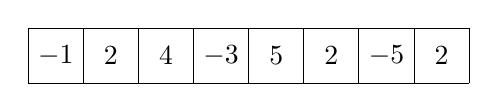
\begin{tikzpicture}[scale=0.7]
\draw (0,0) grid (8,1);

\node at (0.5,0.5) {$-1$};
\node at (1.5,0.5) {$2$};
\node at (2.5,0.5) {$4$};
\node at (3.5,0.5) {$-3$};
\node at (4.5,0.5) {$5$};
\node at (5.5,0.5) {$2$};
\node at (6.5,0.5) {$-5$};
\node at (7.5,0.5) {$2$};
\end{tikzpicture}
\end{center}
\begin{samepage}
o subvetor a seguir produz a soma máxima de $10$:
\begin{center}
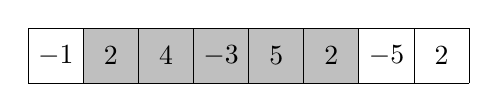
\begin{tikzpicture}[scale=0.7]
\fill[color=lightgray] (1,0) rectangle (6,1);
\draw (0,0) grid (8,1);

\node at (0.5,0.5) {$-1$};
\node at (1.5,0.5) {$2$};
\node at (2.5,0.5) {$4$};
\node at (3.5,0.5) {$-3$};
\node at (4.5,0.5) {$5$};
\node at (5.5,0.5) {$2$};
\node at (6.5,0.5) {$-5$};
\node at (7.5,0.5) {$2$};
\end{tikzpicture}
\end{center}
\end{samepage}

Nós assumimos que um subvetor vazio é permitido, então a soma máxima do subvetor é sempre pelo menos $0$.

\subsubsection{Algoritmo 1}

Uma maneira direta de resolver o problema
é percorrer todos os subvetores possíveis, 
calcular a soma dos valores em cada subvetor e manter 
a soma máxima. 
O código a seguir implementa esse algoritmo:

\begin{lstlisting}
int best = 0;
for (int a = 0; a < n; a++) {
    for (int b = a; b < n; b++) {
        int sum = 0;
        for (int k = a; k <= b; k++) {
            sum += array[k];
        }
        best = max(best,sum);
    }
}
cout << best << "\n";
\end{lstlisting}

As variáveis \texttt{a} e \texttt{b} fixam o primeiro e 
último índice do subvetor, 
e a soma dos valores é calculada na variável \texttt{sum}. 
A variável \texttt{best} contém a soma máxima encontrada durante a busca.

A complexidade de tempo do algoritmo é $O(n^3)$, 
pois consiste em três laços aninhados 
que percorrem a entrada.

\subsubsection{Algoritmo 2}

É fácil tornar o Algoritmo 1 mais eficiente 
removendo um laço dele. 
Isso é possível calculando a soma ao mesmo 
tempo em que o final direito do subvetor se move. 
O resultado é o seguinte código:

\begin{lstlisting}
int best = 0;
for (int a = 0; a < n; a++) {
    int sum = 0;
    for (int b = a; b < n; b++) {
        sum += array[b];
        best = max(best,sum);
    }
}
cout << best << "\n";
\end{lstlisting}
Após essa alteração, a complexidade de tempo é $O(n^2)$.

\subsubsection{Algoritmo 3}

Surpreendentemente, é possível resolver o problema
em tempo $O(n)$\footnote{Em \cite{ben86}, este algoritmo de tempo linear 
é atribuído a J. B. Kadane, e o algoritmo é às vezes 
chamado de \index{algoritmo de Kadane} \key{algoritmo de Kadane}.}, o que significa 
que apenas um loop é necessário.
A ideia é calcular, para cada posição do vetor, 
a soma máxima de um subvetor que termina nessa posição. 
Em seguida, a resposta para o problema é 
o máximo dessas somas.

Considere o subproblema de encontrar o subvetor de soma máxima 
que termina na posição $k$. 
Existem duas possibilidades:
\begin{enumerate}
\item O subvetor contém apenas o elemento na posição $k$.
\item O subvetor consiste em um subvetor que termina 
na posição $k-1$, seguido pelo elemento na posição $k$.
\end{enumerate}

No último caso, uma vez que queremos 
encontrar um subvetor com a soma máxima, 
o subvetor que termina na posição $k-1$ 
também deve ter a soma máxima. 
Portanto, podemos resolver o problema de forma eficiente 
calculando a soma máxima do subvetor 
para cada posição final da esquerda para a direita.

O código a seguir implementa o algoritmo:
\begin{lstlisting}
int best = 0, sum = 0;
for (int k = 0; k < n; k++) {
    sum = max(array[k],sum+array[k]);
    best = max(best,sum);
}
cout << best << "\n";
\end{lstlisting}

O algoritmo contém apenas um laço 
que percorre a entrada, 
portanto, a complexidade de tempo é $O(n)$. 
Essa também é a melhor complexidade de tempo possível, 
porque qualquer algoritmo para o problema 
precisa examinar todos os elementos do vetor pelo menos uma vez.

\subsubsection{Comparação de eficiência}

É interessante estudar como os 
algoritmos são eficientes na prática. 
A tabela a seguir mostra os tempos de execução 
dos algoritmos acima para diferentes 
valores de $n$ em um computador moderno.

Em cada teste, a entrada foi gerada aleatoriamente. 
O tempo necessário para ler a entrada não foi 
medido.

\begin{center}
\begin{tabular}{rrrr}
tamanho do vetor $n$ & Algoritmo 1 & Algoritmo 2 & Algoritmo 3 \\
\hline
$10^2$ & $0.0$ s & $0.0$ s & $0.0$ s \\
$10^3$ & $0.1$ s & $0.0$ s & $0.0$ s \\
$10^4$ & > $10.0$ s & $0.1$ s & $0.0$ s \\
$10^5$ & > $10.0$ s & $5.3$ s & $0.0$ s \\
$10^6$ & > $10.0$ s & > $10.0$ s & $0.0$ s \\
$10^7$ & > $10.0$ s & > $10.0$ s & $0.0$ s \\
\end{tabular}
\end{center}

A comparação mostra que todos os algoritmos 
são eficientes quando o tamanho da entrada é pequeno, 
mas tamanhos maiores de entrada evidenciam 
diferenças notáveis nos tempos de execução dos algoritmos. 
O Algoritmo 1 se torna lento 
quando $n=10^4$, e o Algoritmo 2 
se torna lento quando $n=10^5$. 
Apenas o Algoritmo 3 é capaz de processar 
até mesmo as maiores entradas instantaneamente.
